\documentclass[a4paper]{article}
\usepackage[czech]{babel}
\usepackage[left=2cm,text={17cm,24cm},top=3cm]{geometry}
\usepackage[hidelinks]{hyperref}
\usepackage[utf8]{inputenc}
\usepackage[T1]{fontenc}
\usepackage{listings}
\usepackage{xcolor}
\usepackage[perpage]{footmisc}
\usepackage{graphicx}
\usepackage{todonotes}

\title{Dokumentace návrhu k projektu z předmětu PIS}
\author{Magdaléna Bellayová, Filip Bučko, Hung Do, David Kedra, Matej Matuška}
\date{\today}

\begin{document}

\maketitle
\tableofcontents

\newpage

\section{Tým xdohun00}
\begin{itemize}
    \item Bc. Magdaléna Bellayová (xbella01)
    \item Bc. Filip Bučko (xbucko05)
    \item Bc. Hung Do (xdohun00)
    \item Bc. David Kedra (xkedra00)
    \item Bc. Matej Matuška (xmatus36)
\end{itemize}

\section{Stručný popis informačního systému}
Celý tým se dohodl na tom, že se bude implementovat informační systém pro
\textbf{restauraci}. Naše aplikace lze rozdělit do 4 částí:

\begin{itemize}
    \item \textbf{Webová aplikace pro zákazníky} \\
    Aplikace je cílená pro zákazníky, kteří mají zájem navštívit restauraci. Naleznou tam
    jídelní lístek, otevírací dobu, nebo třeba kontaktní informace.

    \item \textbf{Informační systém pro zaměstnance}  \\
    Zaměstnanec se do systému musí nejprve přihlásit a po přihlášení může vytvářet a
    upravovat rezervace, nebo zadávat objednávky zákazníků. Speciální zaměstnanci (hlavní
    šefkuchaři) mají navíc možnost upravovat menu, přidávat jídla, upravovat ceny a další akce.

    \item \textbf{Manažerský systém} \\
    Manažer bude moci ze systému dostat soupis informací o příjmech a výdajích za dané
    časové období.

    \item \textbf{Administrátorská stránka} \\
    Systém obsahuje speciální roli administrátora, který má na starost přidávání a odebírání
    uživatelských účtů.
\end{itemize}

\newpage

\section{Zvolená architektura systému}
Informační systém bude implementován pomocí třívrstvé architektury. Celá aplikace bude
možná rozjet pomocí předem připraveného \textbf{compose.yaml} souboru, který zapne
všechny potřebné kontejnery. Kontejnery budou primárně spouštěny pomocí aplikace
\textbf{Podman}, nicméně by měly být kompatibilní i s \textbf{Docker}. Jako verzovací
program byl zvolen \textbf{Git} a zdrojové kódy budou ukládány na \textbf{GitHub}.

Vybrané technologie:

\begin{description}
    \item [Datová vrstva:]       MariaDB\footnote{\url{https://mariadb.org/}}
    \item [Aplikační vrstva:]    Jakarta EE Web Profile\footnote{\url{https://jakarta.ee/}} (Java)
    \item [Prezenční vrstva:]    React\footnote{\url{https://react.dev/}} (JavaScript)
\end{description}

\begin{figure}[ht]
    \centering
    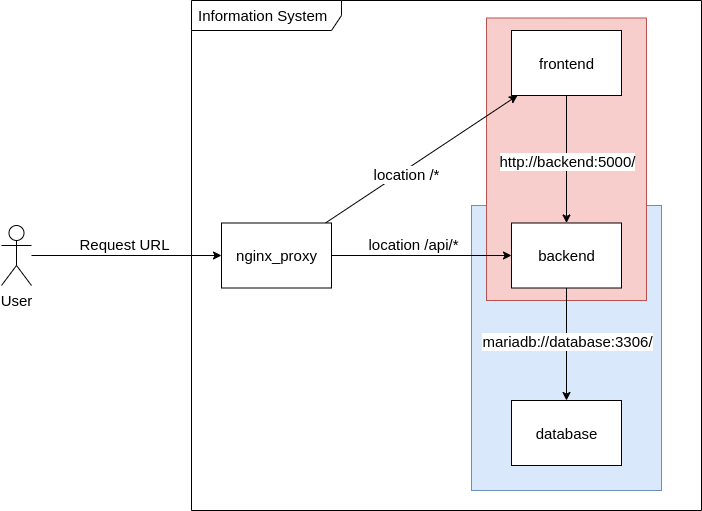
\includegraphics[width=0.9\textwidth]{arch.png}
    \caption{Architektura aplikace.}
\end{figure}

\newpage
\section{Role uživatelů a případy užití}
Se systémem mohou interagovat až 5 aktérů: anonymní uživatel, zaměstnanci (normální zaměstnanec
a hlavní šefkuchař), manažer a administrátor. Jednotlivé případy užití jsou obarvené
podle priority implementace: červená je povinná implementace, modrá a zelená jsou pak
rozšiřující funkcionality, které se mohou implementovat, pokud na to bude čas. Napravo je
pak seznam funkcionalit, které nejsou k žádnému aktéru přiřazené, neboť se neočekává, že
se tyto akce stihnou naimplementovat.

Některé případy užití mají v názvu slovo \emph{manage}. Ve všech těchto případech to
znamená možnost vytvářet nové, zobrazovat, editovat nebo mazat entity.

\begin{figure}[ht]
    \centering
    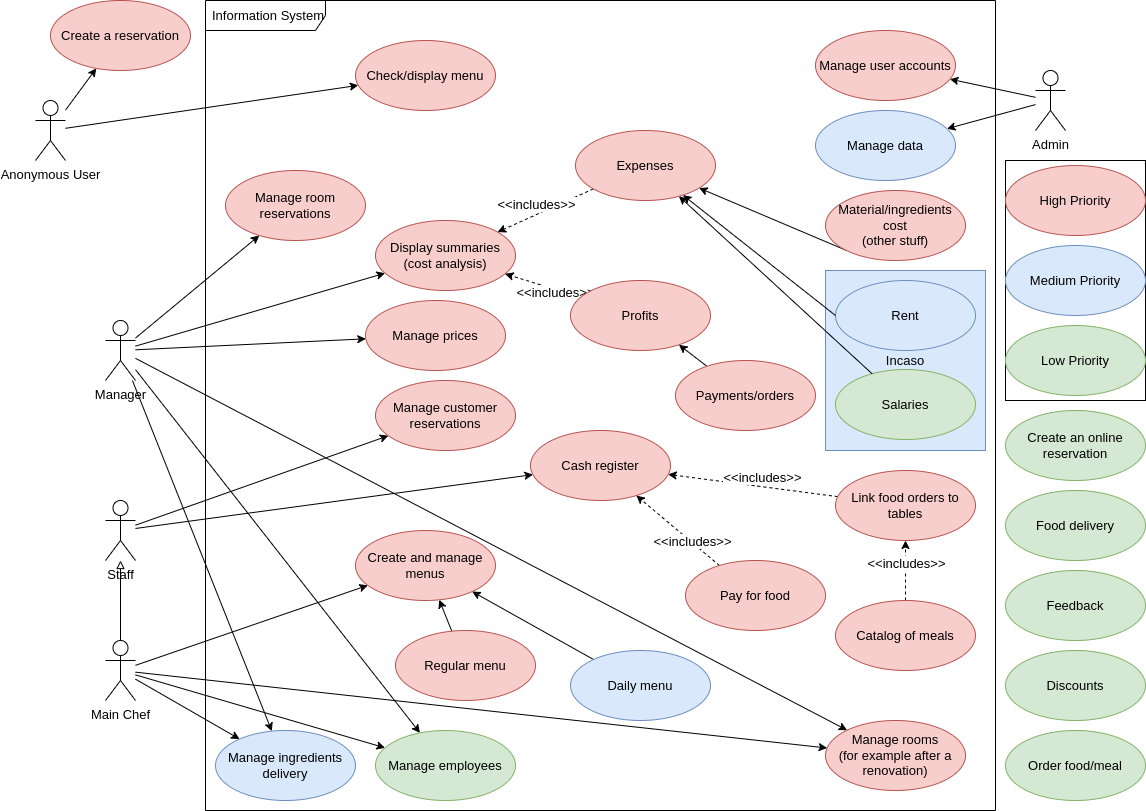
\includegraphics[width=\textwidth]{use_case.png}
    \caption{Případy užití pro jednotlivé uživatele systému.}
\end{figure}

\newpage
\section{Konceptuální datový model}
\begin{figure}[ht]
    \centering
    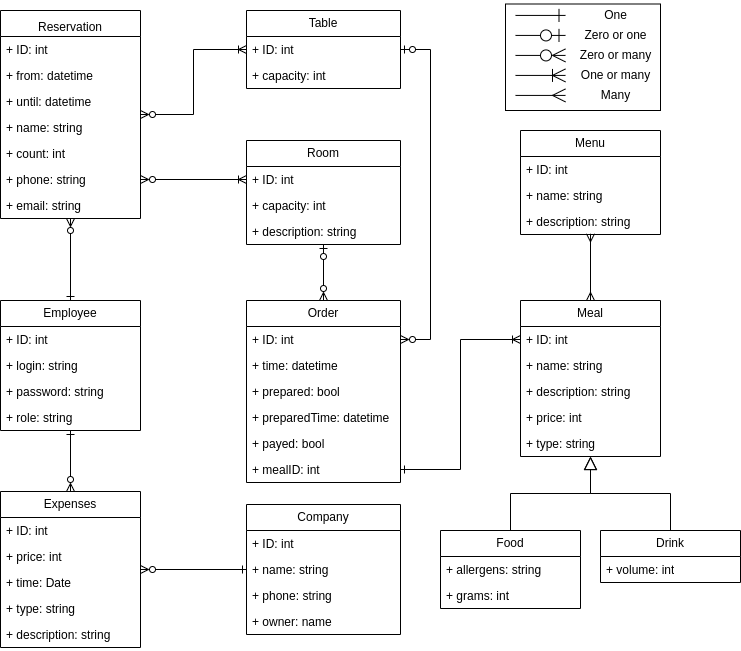
\includegraphics[width=\textwidth]{uml.png}
    \caption{UML diagram systému.}
\end{figure}

\end{document}
